\begin{apendicesenv}
\chapter{BER vs SNR}

Com base na implementação do receptor e transmissor apresentada nas seções \ref{sec:receptor} e \ref{sec:transmissor}, foi realizado um estudo de desempenho do sistema, variando a relação \gls{EbN0} e medindo a \gls{BER} para cada valor, comparando o desempenho do sistema ARGOS-3 com modulação \gls{QPSK} (tanto teórica quanto simulada), conforme apresentado na \autoref{fig:ber_snr}.

\begin{figure}[H]
	\centering
	\caption{Comparação BER vs SNR - ARGOS3 e QPSK}\label{fig:ber_snr}
	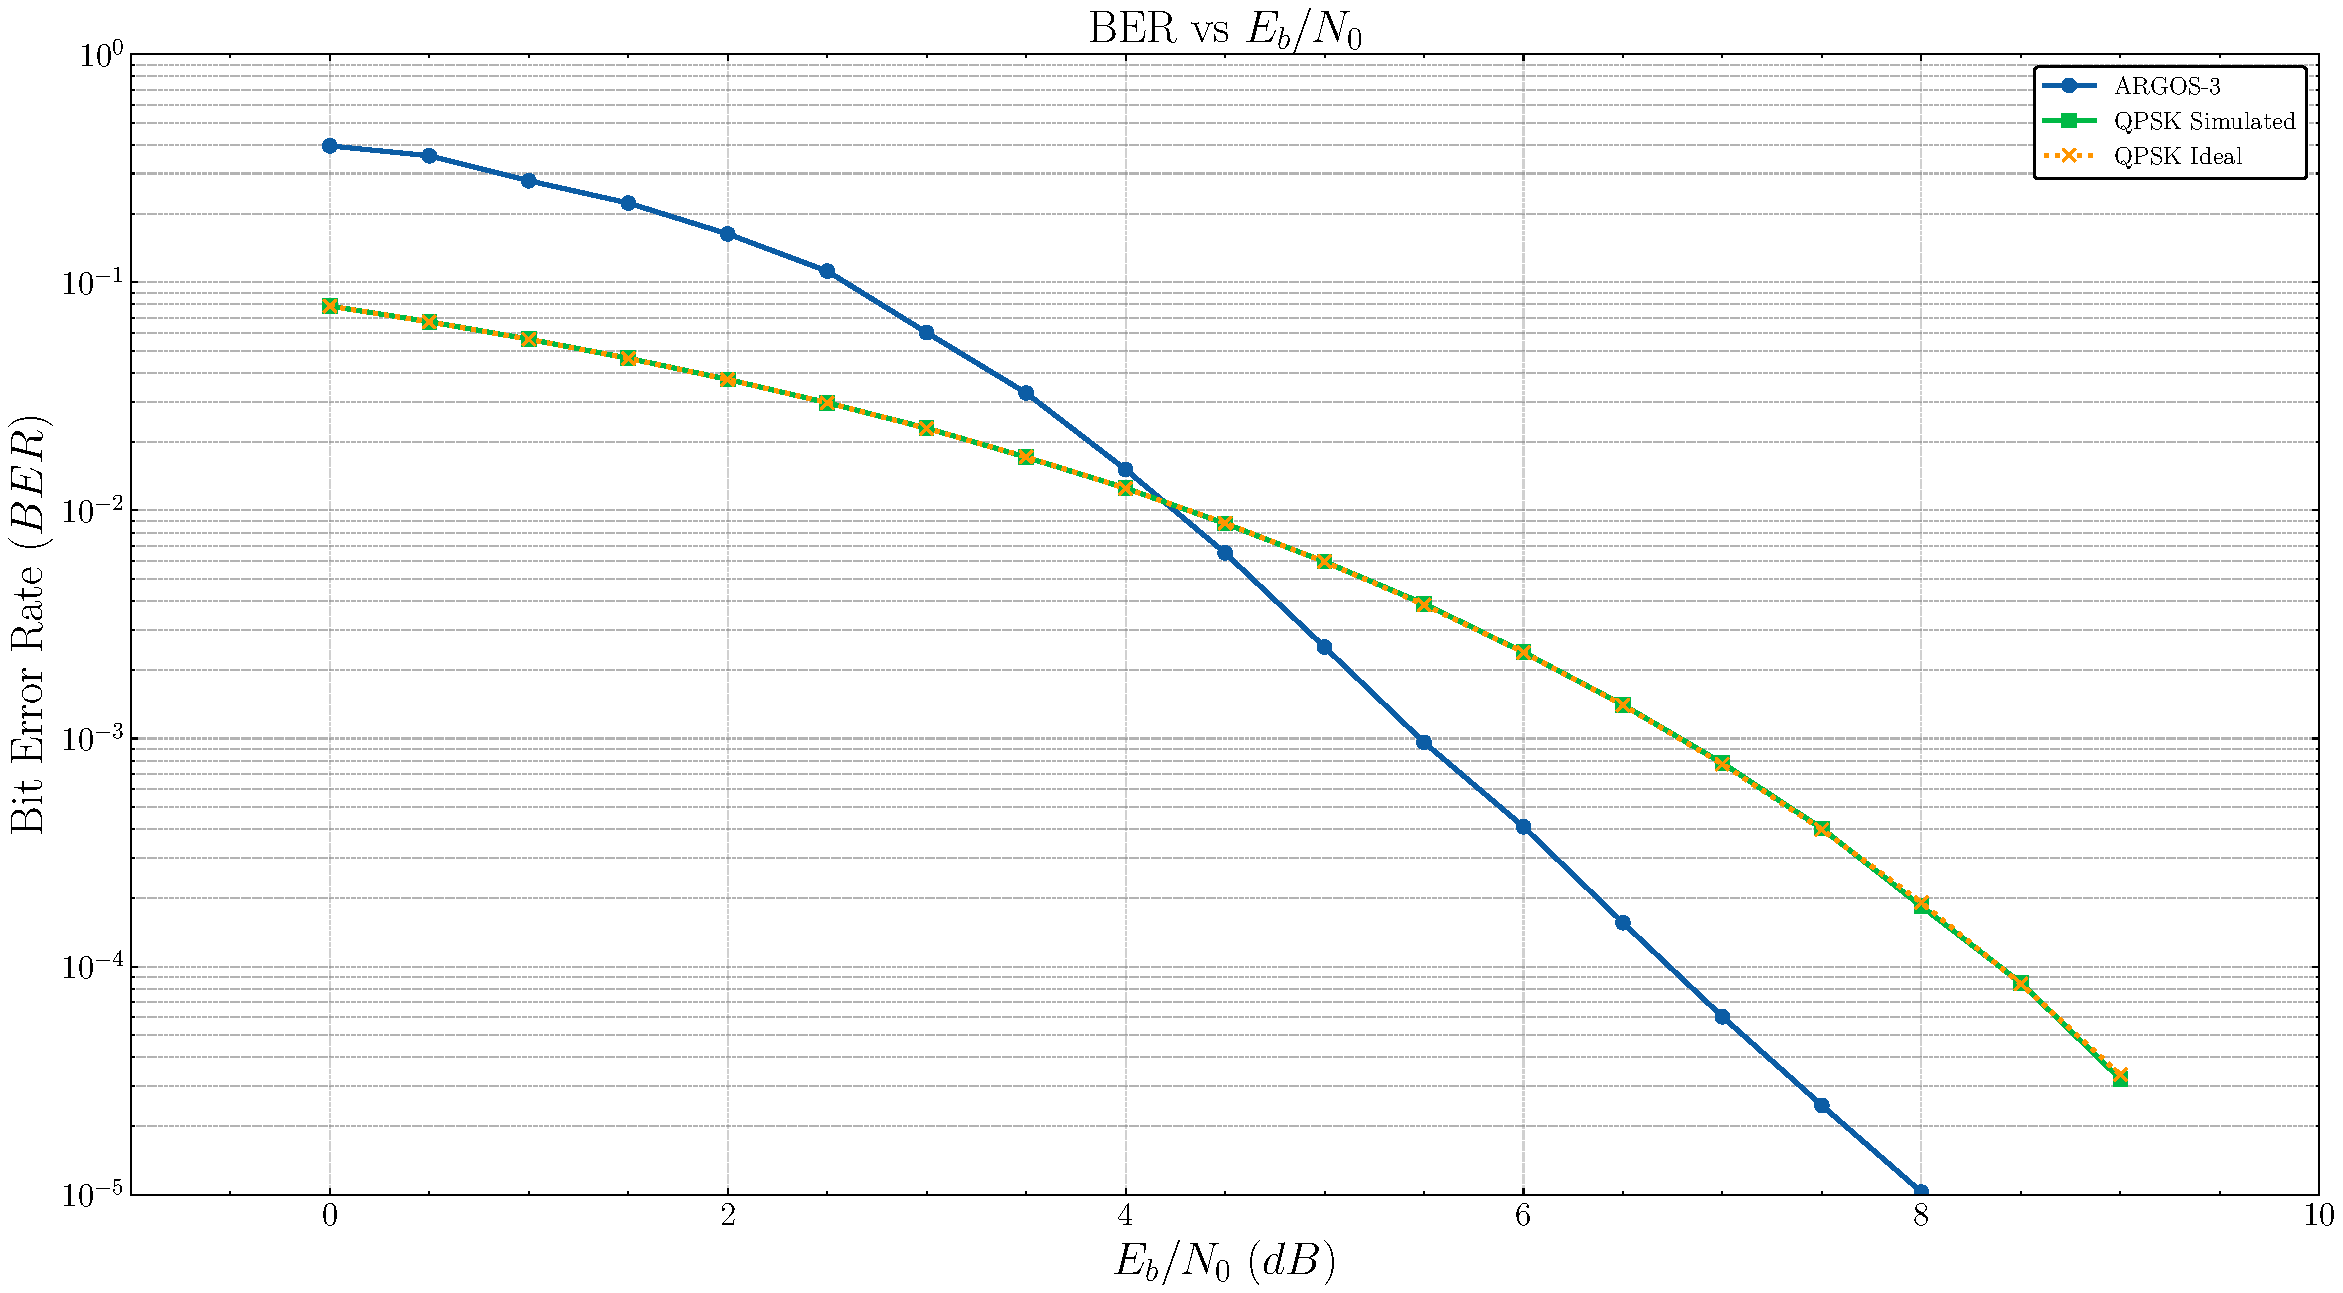
\includegraphics[width=\linewidth]{assets/apendice/ber_vs_ebn0.pdf}
\end{figure}

Nota-se que o desempenho do sistema ARGOS-3 está melhor do que o desempenho teórico e simulado da modulação \gls{QPSK} pura, o que pode ser explicado pela presença do código convolucional, que adiciona redundância aos dados transmitidos, permitindo a correção de erros no receptor, além da presença da técnica de codificação de linha \gls{Manchester}, que também contribui para a melhoria das características do sinal modulado.


\chapter{Simulador OpenSource ARGOS-3}

A implementação do transmissor e receptor ARGOS-3, conforme descrito nas seções \ref{sec:transmissor} e \ref{sec:receptor}, foi realizada em Python, utilizando bibliotecas open source como NumPy, SciPy e Matplotlib. O código-fonte completo do simulador está disponível no repositório GitHub \cite{githubrepository}, permitindo que outros alunos, professores e pesquisadores possam utilizar, modificar e contribuir para o desenvolvimento do projeto. A biblioteca ARGOS-3 utilizada na implementação pode ser instalada via `pip`, conforme mostrado no exemplo de instalação na \autoref{cod:install}. 

\lstinputlisting[language=bash,caption={Exemplo de instalação da biblioteca},label=cod:install]{codigo/install.sh}

O exemplo apresentado no \autoref{cod:argos3} demonstra o uso dos principais módulos da biblioteca, incluindo a criação de um transmissor, a transmissão de um datagrama, a detecção do canal e a recepção do datagrama.

\lstinputlisting[language=python,caption={Exemplo de uso dos principais módulos da biblioteca},label=cod:argos3]{codigo/argos3.py}

\end{apendicesenv}
